\chapter{Marketing}
\begin{flushleft}
    Marketing befasst sich damit ein Produkt unter Menschen zu bringen.
    Dabei soll das Image des Unternehmens erhalten werden.
    Setzt ein Unternehmen Marketing richtig ein, gewinnt und bindet es Kunden.
\end{flushleft}

\section{Marketing-Mix}
\begin{flushleft}
    Der Marketing-Mix besteht aus verschiedenen Marketinginstrumenten, er befasst 
    sich hauptsächlich mit der Umsetzung dieser Instrumente durch Marketingstrategien. \\
    Gänige Marketinginstrumente sind die Produktpolitik, Preispolitik, Vertriebspolitik
    und Kommunikationspolitik. Diese werden auch die vier P's genannt
    (product, price, place, promotion).
\end{flushleft}

\subsection{Produktpolitik}
\subsubsection{Definition}
\begin{flushleft}
    Die Produktpolitik trifft alle Entscheidungen, die das Produkt eines Unternehmens betreffen.
    Beispielsweise entscheidet die Produktpolitik über die Qualität, Funktionalität und das Design
    des Produktes.
\end{flushleft}

\subsubsection{Maßnahmen}
\begin{flushleft}
    Die Produktpolitik orientiert sich an dem \hyperref[subsec:Produktlebenszyklus]{Produktlebenszyklus}
    eines Produktes. Abhängig von der Phase des Produktlebenszyklus nutzt die Produktpolitik eine dieser
    Maßnahmen:
    \begin{enumerate}
        \item {
            \textbf{Produktinnovation} \\
            Das Unternehmen entwickelt neue Produkte um Marktanteile zu bekommen.
        }
        \item {
            \textbf{Produktvariation} \\
            Bestehende Produkte werden weiterentwickelt (``variiert'').
        }
        \item {
            \textbf{Produktelemination} \\
            Produkte, die keine Gewinne mehr abwerfen werden aus dem Portfolio gestrichen.
        }
    \end{enumerate}
\end{flushleft}

\subsection{Preispolitik}
\subsection{Vertriebspolitik}
\subsection{Kommunikationspolitik}

\section{Strategische Analysen}
\subsection{SWOT-Analyse}
\subsection{Produktlebenszyklus}\label{subsec:Produktlebenszyklus}
\begin{flushleft}
    Die Idee hinter dem Produktlebenszyklus ist, dass jedes Produkt einen Lebenszyklus durchläuft.
    Dieser Lebenszyklus wird in fünf verschiedene Phasen eingeteilt.
    Basierend auf der momentanen Phase eines Produktes kann dann abgeschätzt werden, was
    mit diesem Produkt passieren sollte (eliminieren, \dots).
\end{flushleft}

\begin{center}
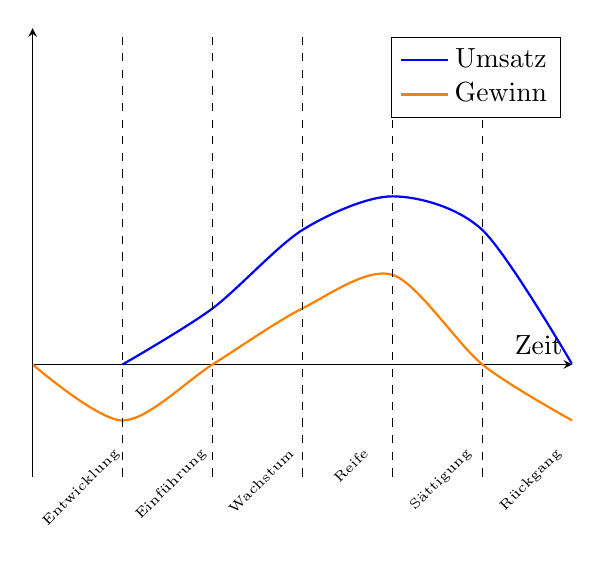
\begin{tikzpicture}
\begin{axis}[
    axis lines=middle,
    xtick=\empty,
    ytick=\empty,
    extra x ticks={1,2,3,4,5,6},
    extra x tick style={major tick length=0pt,yshift=-25pt,xshift=-15pt,opacity=1,grid=none,xticklabel style={font=\tiny ,rotate=45}},
    extra x tick labels={
        Entwicklung,Einführung,Wachstum,Reife,Sättigung,Rückgang
    },
    ymax=3,
    ymin=-1,
    xlabel={Zeit},
    ylabel={\euro}
]
\addplot[blue,smooth,thick] coordinates {
    (1,0) (2,0.5) (3,1.2) (4,1.5) (5,1.2) (6,0)
};
\addlegendentry{Umsatz}
\addplot[orange,smooth,thick] coordinates {
    (0,0) (1,-0.5) (2,0) (3,0.5) (4,0.8) (5,0) (6,-0.5)
};
\addlegendentry{Gewinn}
\draw[color=black, dashed] (axis cs:1, -1) -- (axis cs:1, 3);
\draw[color=black, dashed] (axis cs:2, -1) -- (axis cs:2, 3);
\draw[color=black, dashed] (axis cs:3, -1) -- (axis cs:3, 3);
\draw[color=black, dashed] (axis cs:4, -1) -- (axis cs:4, 3);
\draw[color=black, dashed] (axis cs:5, -1) -- (axis cs:5, 3);
\end{axis}
\end{tikzpicture}
\end{center}
\pagebreak

\begin{flushleft}
    Jede Phase verfügt über verschiedene Merkmale.
\end{flushleft}
\begin{center}
\begin{tabular}{|l|p{8cm}|}
    \hline
    \textbf{Phase} & \textbf{Merkmale} \\
    \hline
    Entwicklung & Das Produkt befindet sich noch in der Entwicklung und deshalb noch nicht auf dem Markt. Es hat bisher nur Kosten verursacht. \\
    \hline
    Einführung & Das Produkt wird in den Markt eingeführt. Dabei entstehen jedoch hohe Kosten durch Werbung. Zum Ende dieser Phase sollte das Produkt die Kosten decken können. \\
    \hline
    Wachstum & In der Wachstumsphase steigt der Umsatz des Produktes stark an. Der Markt ist jedoch noch stark umkämpft, deshalb bleiben hohe Werbekosten. \\
    \hline
    Reife & Die Reifephase zeigt hohe Gewinne während der Umsatz weniger steigt als in der Wachstumsphase. Nach der Reifephase fallen Gewinn und Umsatz. \\
    \hline
    Sättigung & In der Sättigungsphase fallen Umsatz und Gewinn, zum Ende dieser Phase wird meist kein Gewinn mehr erzielt. \\
    \hline
    Rückgang & In der Phase des Rückgangs oder der Degeneration macht das Produkt Verlust. Es ist die letzte Phase des Produktlebenszyklus und damit das Ende des Produktes. \\
    \hline
\end{tabular}
\end{center}

\subsection{Portfolioanalyse (BCG-Matrix)}
\begin{flushleft}
    Die Portfolioanalyse ist eine Analysestrategie, die eine übersichtliche Darstellung des gesamten
    Portfolio erlaubt. Bei einer Portfolioanalyse wird eine Vierfeldmatrix erstellt, diese Matrix wird auch BCG-Matrix
    genannt, da sie durch die Boston Consulting Group bekannt wurde. Die vier Felder stellen die vier Produktlebensphasen dar.
\end{flushleft}
\begin{center}
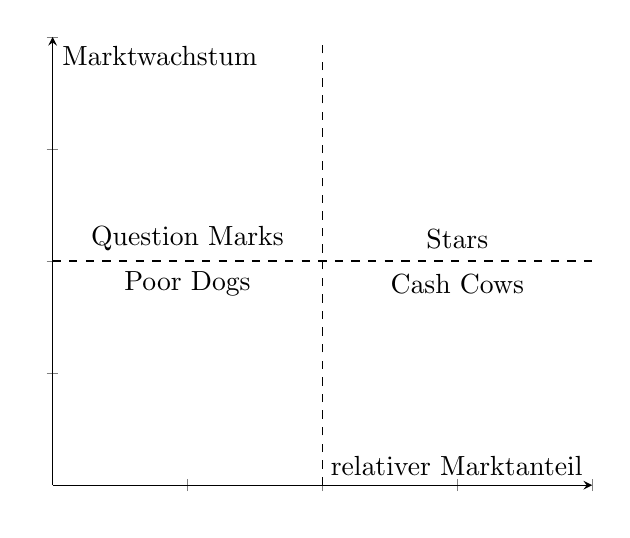
\begin{tikzpicture}
\begin{axis}[
    axis lines=middle,
    xlabel={relativer Marktanteil},
    ylabel={Marktwachstum},
    xmax=2,
    xmin=0,
    ymax=2,
    ymin=0,
    xticklabel=\empty,
    yticklabel=\empty
]
\addplot[draw=none] coordinates {
    (0,0)
};
\draw[color=black, dashed] (axis cs:0, 1) -- (axis cs:2, 1);
\draw[color=black, dashed] (axis cs:1, 0) -- (axis cs:1, 2);
\draw (axis cs:0.5,1.1) node {Question Marks};
\draw (axis cs:1.5,1.1) node {Stars};
\draw (axis cs:0.5,0.9) node {Poor Dogs};
\draw (axis cs:1.5,0.9) node {Cash Cows};
\end{axis}
\end{tikzpicture}
\end{center}

\begin{flushleft}
    So wie bei dem Produktlebenszyklus gibt es hier verschiedene Merkmale für die Produktlebensphasen.
\end{flushleft}
\begin{center}
\begin{tabular}{|l|p{8cm}|}
    \hline
    \textbf{Phase} & \textbf{Merkmale} \\
    \hline
    Question Marks & Question Marks haben ein hohes Marktwachstum aber einen kleinen relativen Marktanteil. Es muss entschieden werden ob es sich lohnt den relativen Marktanteil durch Vermarktung zu steigern oder nicht. \\
    \hline
    Stars & Die Stars des Portfolios haben ein hohes Marktwachstum und einen hohen relativen Marktanteil. Sie befinden sich in der optimalen Position. \\
    \hline
    Poor Dogs & Alle neuen Produkte sind zu erst Poor Dogs. Alte Produkte, die keine Gewinne mehr abwerfen werden zu Poor Dogs. \\
    \hline
    Cash Cows & Da Cash Cows einen hohen relativen Marktanteil aber ein niedriges Marktwachstum haben, wird versucht aus ihnen das meiste herauszuholen. Sie werden wie Kühe gemolken. \\
    \hline
\end{tabular}
\end{center}

\section{Marktforschung}